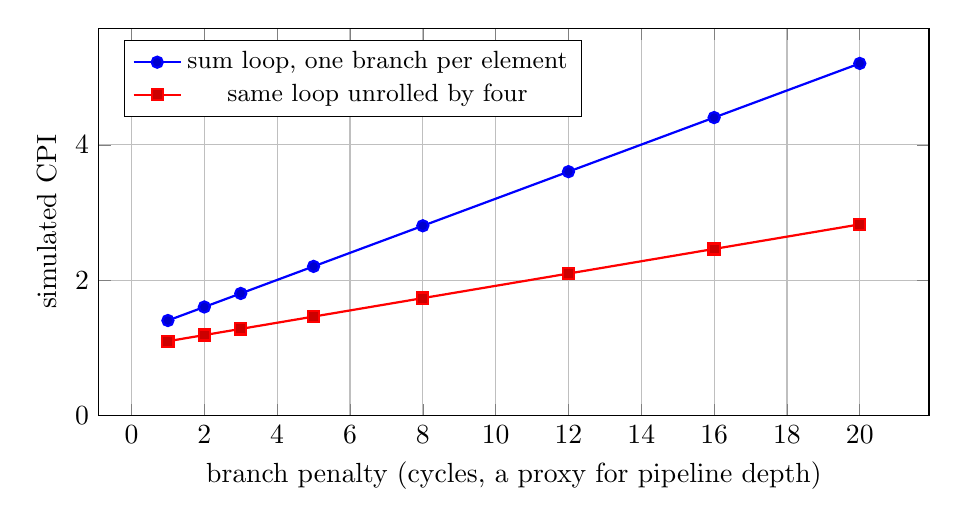
\begin{tikzpicture}
\begin{axis}[width=\textwidth, height=6.5cm, xlabel={branch penalty (cycles, a proxy for pipeline depth)}, ylabel={simulated CPI}, grid=major, ymin=0, legend pos=north west, legend style={font=\small}]
\addplot+[mark=*, thick] coordinates {(1,1.404) (2,1.604) (3,1.804) (5,2.204) (8,2.804) (12,3.604) (16,4.404) (20,5.204)};
\addlegendentry{sum loop, one branch per element}
\addplot+[mark=square*, thick] coordinates {(1,1.098) (2,1.189) (3,1.28) (5,1.462) (8,1.735) (12,2.098) (16,2.462) (20,2.825)};
\addlegendentry{same loop unrolled by four}
\end{axis}
\end{tikzpicture}